% $Id$

\chapter{Multiple Kernel Learning Example}
\label{data_example3}
\minitoc


This chapter will describe the steps necessary to perform a classification with SimpleMKL \url{http://asi.insa-rouen.fr/enseignants/~arakoto/code/mklindex.html} \cite{Rakotomamonjy2008} using PRoNTo. These are similar to the ones in Chapter \ref{sec:Block_design_fMRI_dataset}, thus, the reader is advised to complete the tutorial in Chapter \ref{sec:Block_design_fMRI_dataset}  before moving on, since the explanation of some steps will be less descriptive.

Many practical learning problems involve multiple and heterogeneous data sources. In this way, Multiple Kernel Learning (MKL) \cite{Bach2004} has been proposed to simultaneously learn and combine different models, represented by different kernels, in supervised learning settings. In MKL, the kernel $K$  can  be  considered  as  a  linear  combination  of $M$ `basis kernels'. For further details, please refer to \cite{Bach2004}.

One example of a MKL approach based on SVM is the SimpleMKL algorithm \cite{Rakotomamonjy2008}. Essentially, the algorithm is based on a gradient descent on the SVM objective value and iteratively determine the combination of kernels by a gradient descent wrapping \cite{Rakotomamonjy2008}. For further details, please refer to \cite{Rakotomamonjy2008}

We will use the same dataset used in Chapter \ref{sec:Block_design_fMRI_dataset}, this fMRI dataset originates from a study on face and object representation in human ventral temporal cortex \cite{Haxby2001}. The dataset\footnote{Pre-processed (realigned and normalised) data from participant 1.} used in this chapter can be found in PRoNTo's website \url{http://www.mlnl.cs.ucl.ac.uk/pronto/prtdata.html} (data set 1) and the whole\footnote{Not pre-processed.} dataset is available in \url{http://data.pymvpa.org/datasets/haxby2001/}.

For simplicity, in this example we will use PRoNTo to predict if the subject is viewing an image of a Face or a House based on the fMRI scans. We will classify the whole brain images using SimpleMKL and a leave one block out cross-validation scheme.

\section{GUI analysis}

We will first analyse the data using PRoNTo's GUI and then repeat the analysis using the {\tt matlabbatch} system.

To start, create a new directory in which to save the results of the analysis, then start up MATLAB and type `prt' or `pronto' in the MATLAB prompt. This will open the main interface of PRoNTo (Figure \ref{fig:mainInterfacemkl}).

\begin{figure}[!h]
	\centering
		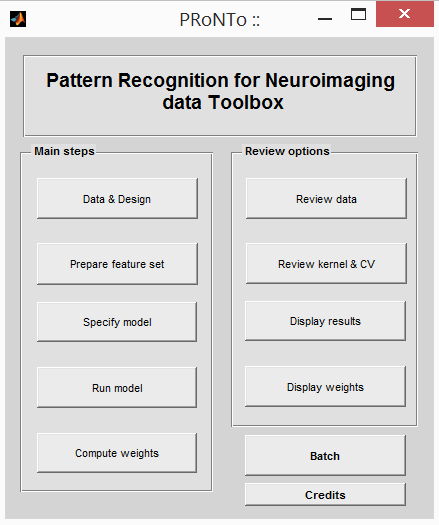
\includegraphics[scale=0.75]{images/Tutorial/mkl/mainInterfacemkl.png}
	\caption{Main interface of PRoNTo.}
	\label{fig:mainInterfacemkl}
\end{figure}

%--------------------------------------------------------------------------

\subsection{Data \& Design}


\begin{itemize}
	
	\item In PRoNTo's main window, click on `Data \& Design'. Like in the previous chapters, browse the directory in which to save the PRT structure (saved as `PRT.mat');
	
	\item In the panel `Groups', click on `Add' and provide a name to the group (we only have one group/subject), with no spaces, e.g. `G1';
	
	\item Add a subject in the `Subject/Scans' option, e.g. `S1', and leave the `Scans' tick box below the panel unchecked. See Chapter \ref{chap:DataDesign} of the manual for more information on this option;
	
	\item In the `Modalities' panel, click on `Add' and provide a name to the modality, e.g. `fMRI'. In the `Design' field, choose the option `Load SPM.mat'. This file is available with the Haxby dataset on PRoNTo's website\footnote{http://www.mlnl.cs.ucl.ac.uk/pronto/prtdata.html} inside the folder Haxby\_dataset/design/;
	

	\begin{itemize}
	
		\item In case there is no `SPM.mat' file available to use, create a new design by selecting the option `Specify design'. Choose how many conditions you have, which in this case are 8 conditions (corresponding to the 8 categories of images). This will open another window that allows the user to write the names, onsets and durations (if the duration is the same for all events only one value is required) of each condition. The unit in which the onsets/durations are read in this case is `scans' and the interscan interval (TR) is 2.5 seconds. The design information (names, onsets and durations) can be found inside the `Haxby\_design.pdf' file in the Haxby dataset folder. 
	
	\end{itemize}
	
	
	\item Finally, load all the image files available in the fMRI directory (Haxby\_dataset/fMRI/). You can select all the files by using the right mouse button and clicking on the option `Select All'. When all the images are selected, click on the `Done' button;
	
	\item In the `Masks' field, on the bottom left of the `Data and design' window, select the `whole\_brain' mask for the specified modality. The mask is available in the masks directory inside the folder Haxby\_dataset/masks/;

	\item Click on the 'Review' button to check the data and the design inserted for this modality. For more information on what one can do with the Review option, please see Chapter \ref{chap:DataDesign};
	
	\item The `Data and design' window should look similar to the one in Figure \ref{fig:dataDesignmkl}. Click on the 'Save' button to create the `PRT.mat' file with the structure containing the information that has been previously specified. If no errors are shown in the MATLAB command, leave the `Data and design' window by clicking `Quit'.
	

\begin{figure}[!h]
	\centering
		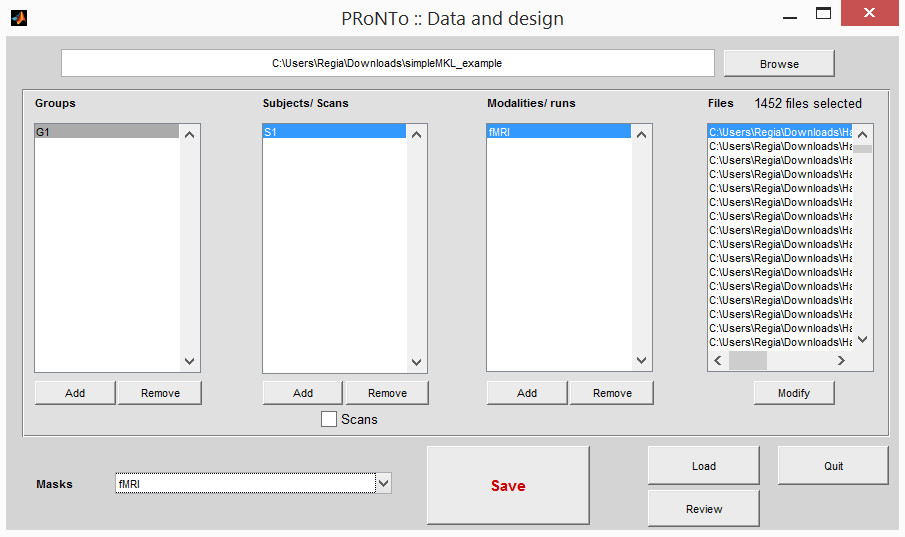
\includegraphics[scale=0.7]{images/Tutorial/mkl/dataDesignmkl.png}
	\caption{`Data and design' GUI final configuration.}
	\label{fig:dataDesignmkl}
\end{figure}	

\end{itemize}

%--------------------------------------------------------

\subsection{Prepare feature set}

\begin{itemize}
	
	\item In PRoNTo's main window, click on `Prepare feature set' and a new window called `Prepare feature set' will open (see Figure \ref{fig:prepareFeature} in Chapter \ref{sec:Block_design_fMRI_dataset});
	
	\item Select the `PRT.mat' file previously created in the `Data \& Design' step and another window will open, `Specify modality to include' (see Figure \ref{fig:specifyModality} in Chapter \ref{sec:Block_design_fMRI_dataset}), to set the specification of different parameters and options for each modality, which are: 
	
	\begin{itemize}
		\item `Modality' field: select the modality previously specified in the `Data \& Design' step, `fMRI';

		\item `Conditions' field: select `All scans'; 
		
		\item `Parameters' box: select the polynomial detrend with order 1 and the 'No scaling' option;
		\item `Features' box: select the `Build one kernel per region' tick box and load the `AAL' atlas (named 'aal\_79x91x69') available in the PRoNTo directory (PRoNTo/atlas/). Then, click on the 'Done' button. The final `Specify modality to include' window should look similar to the one in Figure \ref{fig:specifyModalitymkl};
		
			
		\begin{figure}[!h]
	\centering
		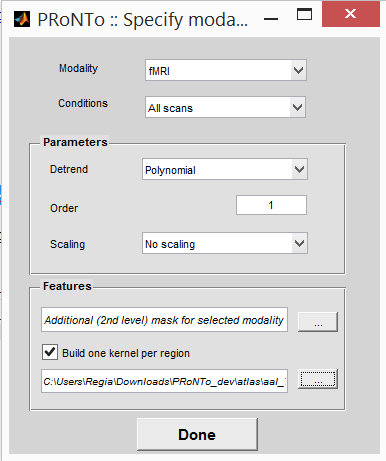
\includegraphics[scale=0.75]{images/Tutorial/mkl/specifyModalitymkl.png}
	\caption{`Specify modality to include' GUI final configuration.}
	\label{fig:specifyModalitymkl}
\end{figure}	
		
			%\begin{itemize}
			%\item As an optional step, in the `Additional mask for selected modality' field, the user can specify a `second-level' mask, which can be used to select regions of interest (ROIs) in which the classification can be performed. For instance, we can enter the `fusiform\_gyrus' mask available with this dataset; 
			%\end{itemize}	
			
		
	\end{itemize}		
		
	\item In the `Prepare feature set' window, provide a name to the feature set, e.g. `HaxbyFeatures';

	\item Click on `Build kernel/data matrix' to build the feature set and kernel. It will take a few minutes.

\end{itemize}


%---------------------------------------------------------------------

\subsection{Specify model}

\begin{itemize}
	
	\item In PRoNTo's main window, click on `Specify model' and a new window called `Specify model' will open (see Figure \ref{fig:specifyModel} in Chapter \ref{sec:Block_design_fMRI_dataset});
	
	\item Select the `PRT.mat' file and provide a name to the model, e.g. `mklFacesHouses';

	\item Select one of the feature sets previously defined. In this case, there is only one: `HaxbyFeatures';

	\item Leave the option `Use kernels' tick box as it is, i.e. `Yes';

	\item	Select the `Classification' model type and click on the 'Define classes` button. A new window will open, `Specify classes', to define the number of classes and a name for each class. We will define 2 classes:
	
		\begin{itemize}
			\item for `Class 1' select subject `S1' and the condition `Faces' and;
			\item for `Class 2' select subject `S1' and the condition `Houses'. Click on `Done'.
		\end{itemize}		
	  
	
	\item Select the `L1- Multi-Kernel Learning' option, in the Machine field;
	
	\item Select the `Optimize hyper-parameter' tick box and leave the textbox empty. This will force PRoNTo to use an array with default hyper-parameter values for the optimization. You can choose other values by inputing them in this box (e.g. [0.1, 1, 100]);
	
	\item In the `Cross-Validation Scheme' (internal loop) field, select the option `k-fold CV on Block'. A window will appear asking to define the value of k, set it to 4;
		
	\item Select the `Leave One Block Out' cross-validation scheme (external loop); 
	
	\item In the `Data operations' box, select the `Mean centre features using training data' and `Normalize samples' options Then, the `Specify model' window should look similar to the one in Figure \ref{fig:specifyModelmkl};
	
	\begin{figure}[!h]
	\centering
		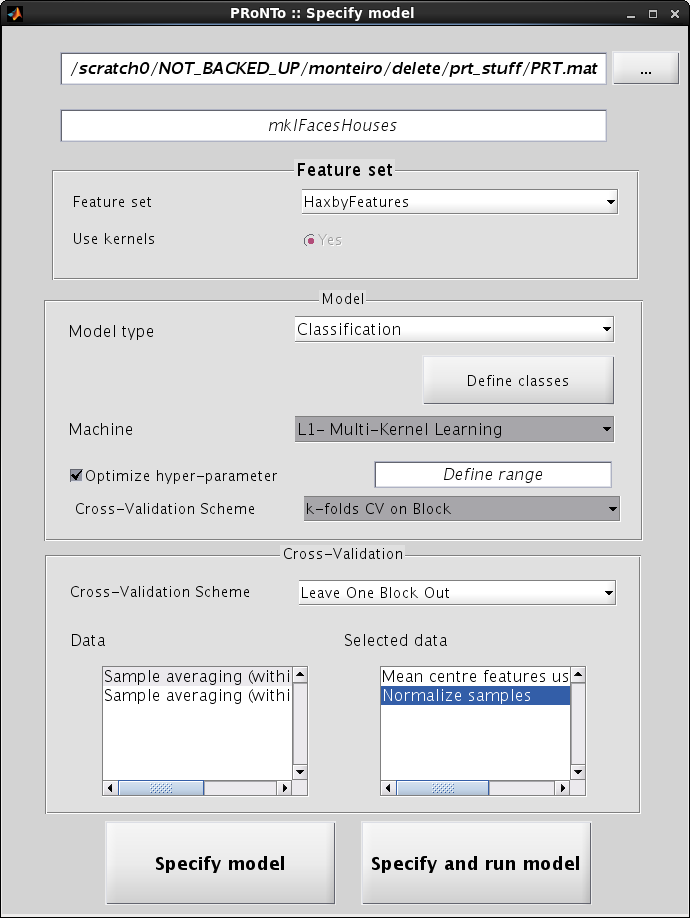
\includegraphics[width=0.7\textwidth]{images/Tutorial/mkl/specifyModelmkl.png}
	\caption{`Specify model' GUI final configuration.}
	\label{fig:specifyModelmkl}
\end{figure}
	
	\item Click on `Specify and run model' and the model will be immediately estimated, therefore there is no need to use the `Run model' module in this case. It will take a few minutes to complete.

\end{itemize}

%--------------------------------------------------------------------

\subsection{Display model (optional step)}

\begin{itemize}
\item To review the model specification, in the main PRoNTo GUI, click on `Review kernel \& CV' and a new window will open, `Review Model Specification' (see Figure \ref{fig:reviewModel} in Chapter \ref{sec:Block_design_fMRI_dataset});


\item Select the model, `mklFacesHouses', from the list at the top and click on `Review model'; then, select one class from the list to see which groups, subjects and conditions belong to this class (see Figure \ref{fig:reviewModelClass} in Chapter \ref{sec:Block_design_fMRI_dataset});


\item To review the data and cross-validation matrix click on `Review CV' (Figure \ref{fig:reviewCVmkl}). For more information on what these matrices mean, please consult the previous chapters of the manual;

\begin{figure}[!h]
	\centering
		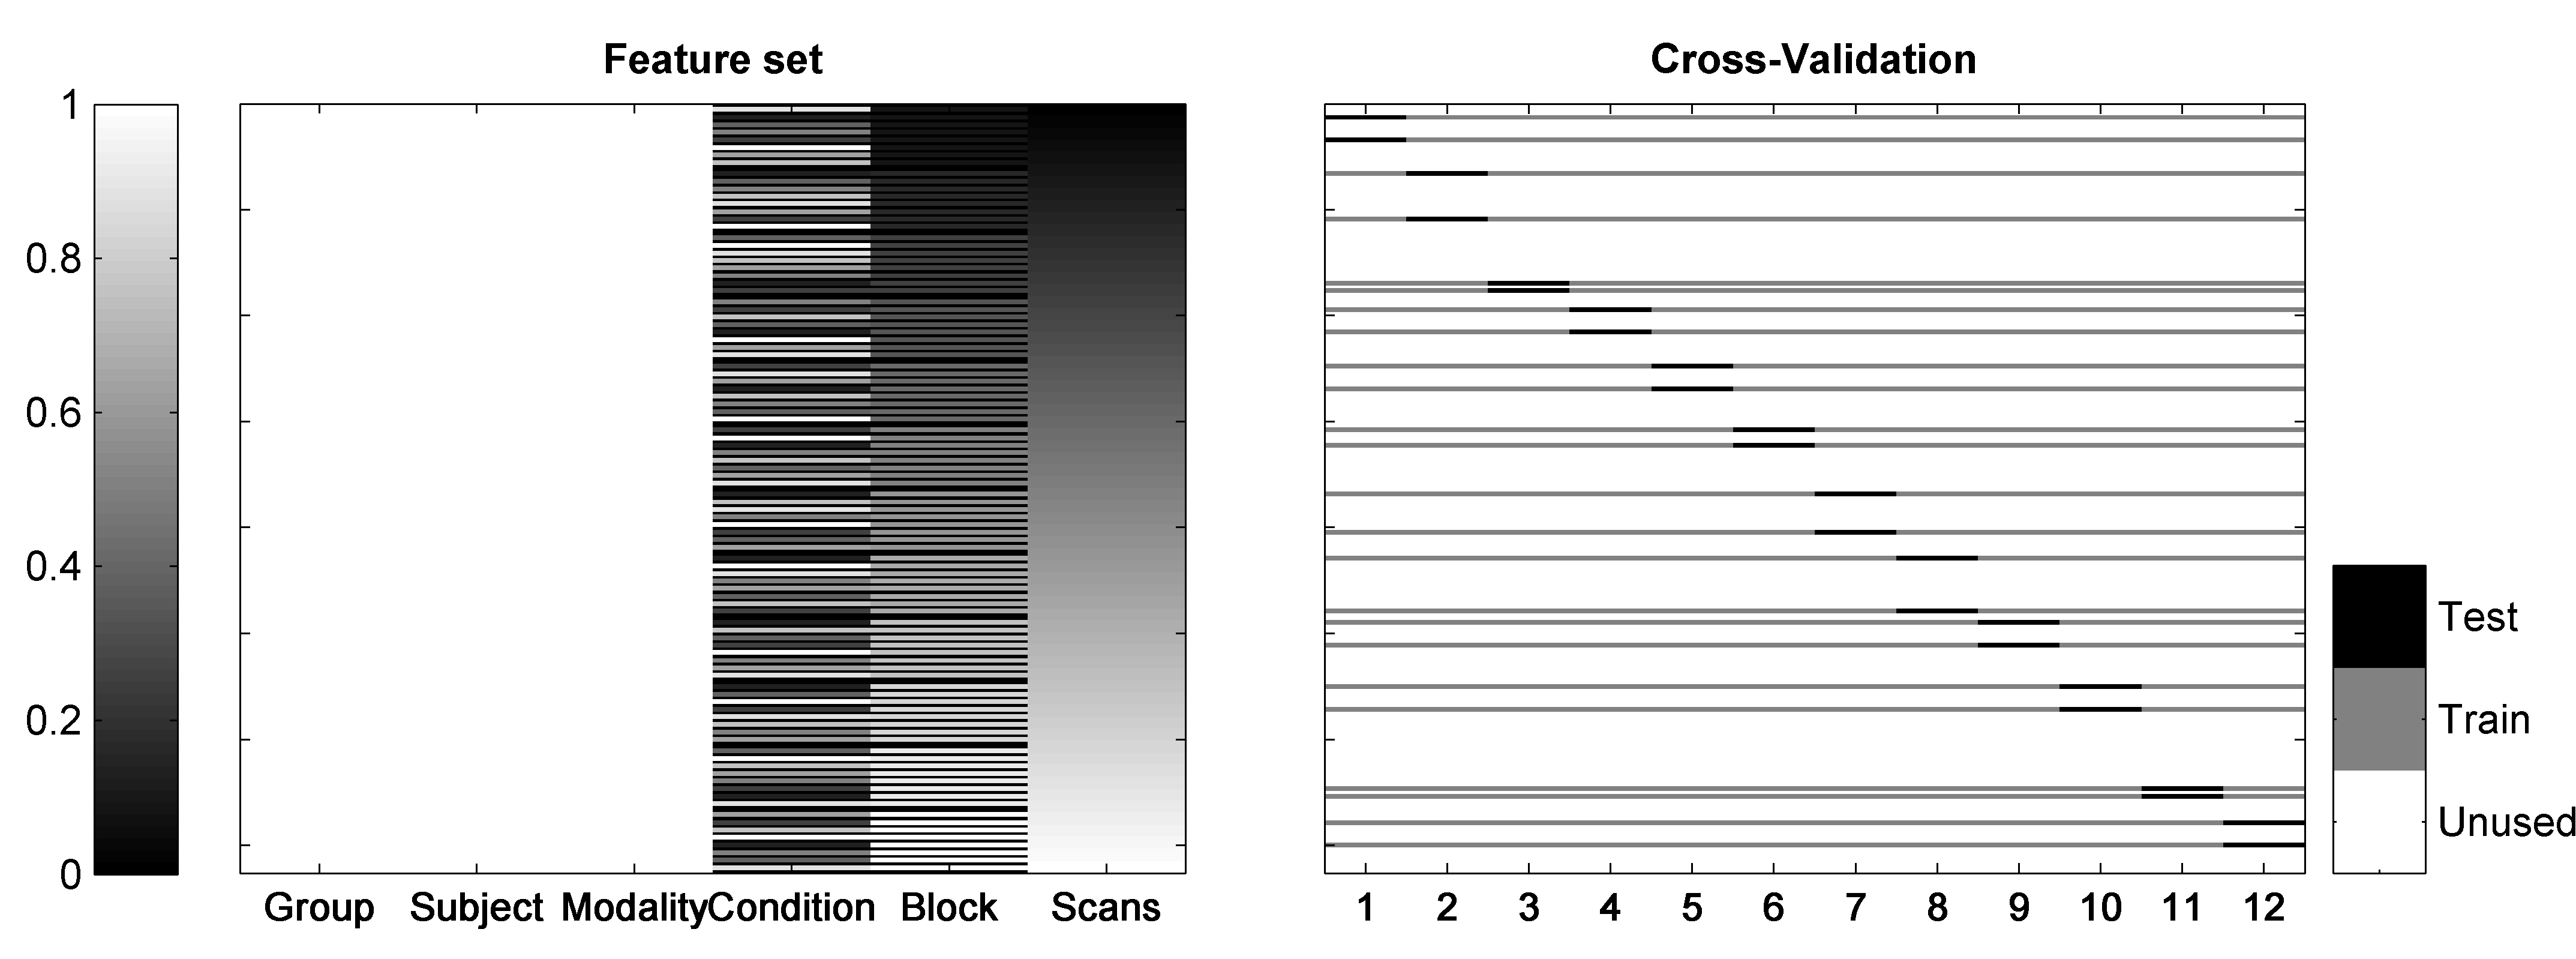
\includegraphics[scale=0.7]{images/Tutorial/mkl/reviewCVmkl.png}
	\caption{Data and cross-validation matrix from `Review CV' option.}
	\label{fig:reviewCVmkl}
\end{figure}

\item To review the kernel, click on `Show kernel' (Figure \ref{fig:reviewKernelmkl}).

\begin{figure}[!h]
	\centering
		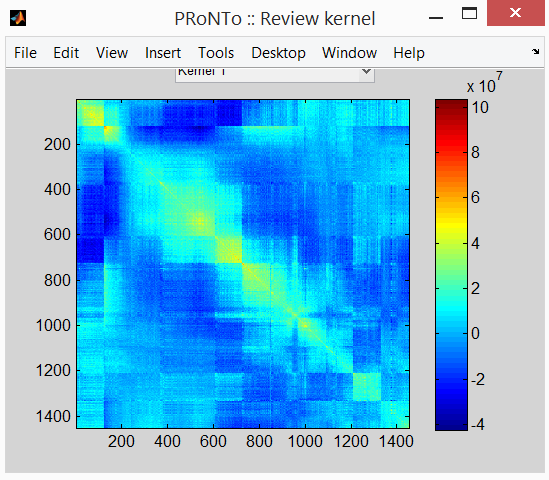
\includegraphics[scale=0.7]{images/Tutorial/mkl/reviewKernelmkl.png}
	\caption{Kernel matrix used for classification.}
	\label{fig:reviewKernelmkl}
\end{figure}

\end{itemize}

%----------------------------------------------------

\subsection{Compute weights (optional step)}

\begin{itemize}
\item In PRoNTo's main window, click on `Compute weights' and a new window will open, `Compute weights' (see Figure \ref{fig:computeWeights} in Chapter \ref{sec:Block_design_fMRI_dataset}); 

\item Select the `PRT.mat' file;

\item Select the model from the list to `Models computed in PRT', `mklFacesHouses' model;

\item Check the tick box option `Compute average/kernel weight per region';

\item Click on the 'Compute weights' button. Computations will be displayed on the MATLAB prompt.

\end{itemize}

%------------------------------------------------------------------

\subsection{Display results}
\label{display_results_MKL}

\begin{itemize}
	
	\item In PRoNTo's main window, click on `Display results' and select the `PRT.mat' file. This will open the main results window. In the `Model' panel, select the model that you want to view, `mklFacesHouses', and the results through performance will be similar to the one in Figure \ref{fig:resultsmkl};
	
	\begin{figure}[!h]
	\centering
		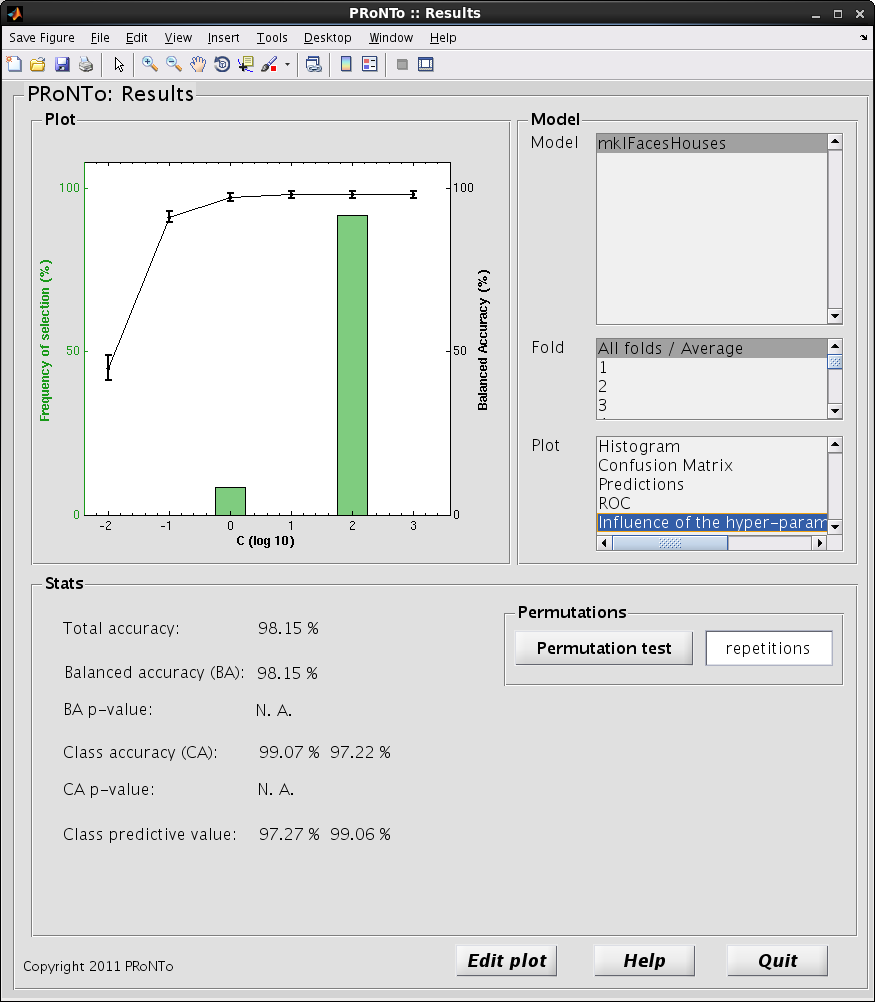
\includegraphics[width=0.75\textwidth]{images/Tutorial/mkl/resultsmkl.png}
	\caption{Summary for model's performance.}
	\label{fig:resultsmkl}
\end{figure}
	
	\item In the `Results' window, one can select the different plots in the `Plots' list. Please note that there is a new plot on the list, this displays information about the hyper-parameter optimization, for more information, please refer to Chapter \ref{chap:DisRes}.
		
	
\end{itemize}
	
%------------------------------------------------------------------

\subsection{Display weights}

\begin{itemize}
	
	\item In PRoNTo's main window, click on `Display weights' and select the `PRT.mat' file. This will open the `Model interpretation' window. By clicking on `Model', mklFacesHouses, an image will appear in the `Weights map' box; and to show the `Anatomical img' you have to load an anatomical image for reference. A template image can be found in the SPM's canonical folder `single\_subj\_T1'. The final result window will look similar to that shown in Figure \ref{fig:modelInterpretationMKL}.

    \item Since the machine used in the example was MKL with a kernel calculated for each brain region, it is possible to see the contributions of each region. The labels for the regions can be found in the same folder where the atlas is located (PRoNTo/atlas). For more information, please refer to Chapter \ref{chap:DisWeights}.

\begin{figure}[!h]
	\centering
		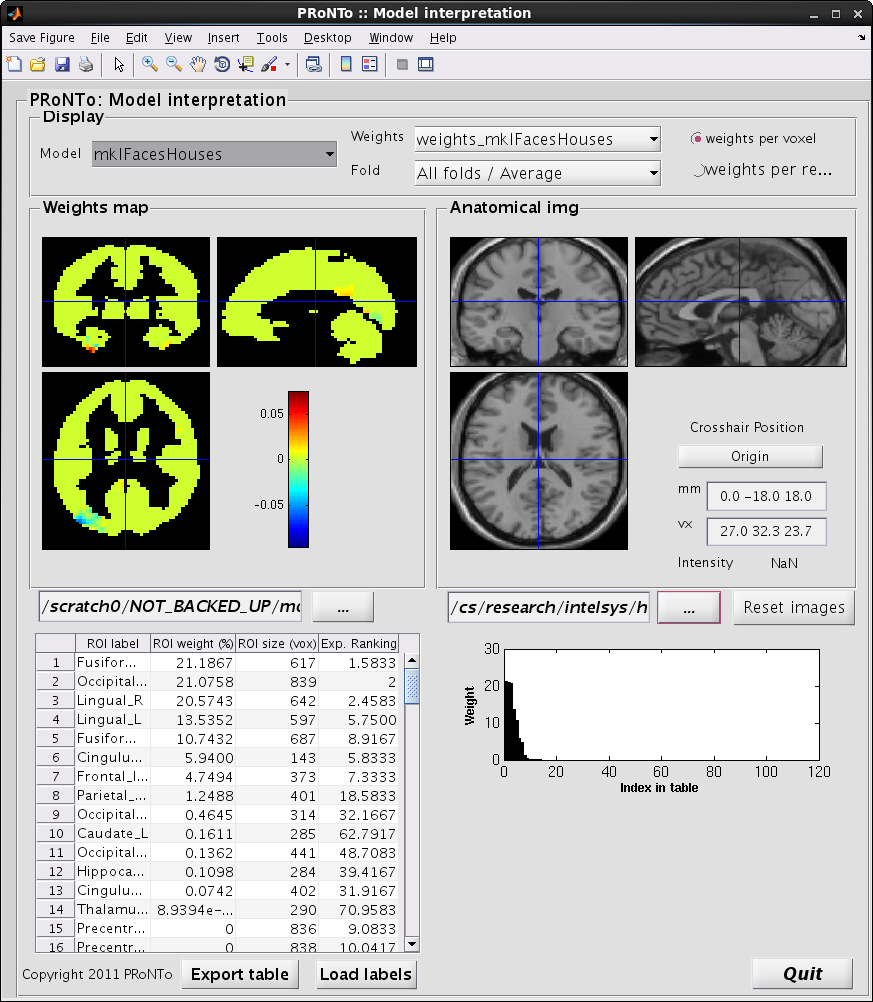
\includegraphics[width=0.75\textwidth]{images/Tutorial/mkl/modelInterpretationMKL.png}
	\caption{Summary for model's performance.}
	\label{fig:modelInterpretationMKL}
\end{figure}
	
\end{itemize}

%=====================================================



%=====================================================

\section{Batch analysis}
\label{sec:Batch_analysis}

This tutorial will now show how to analyse the same data but using the {\tt matlabbatch} system.

Once again, to analyse the data, create a new directory in which to save the results of the analysis, saved as 'PRT.mat'. On the main interface of PRoNTo click on the 'Batch' button to open the `{\tt matlabbatch}'. Alternatively, type `prt\_batch' in the MATLAB prompt. On the menu bar of the batch, there is a PRoNTo menu with the 5 options shown in the main steps interface (Figure \ref{fig:batchmkl}).

\begin{figure}[!h]
	\centering
		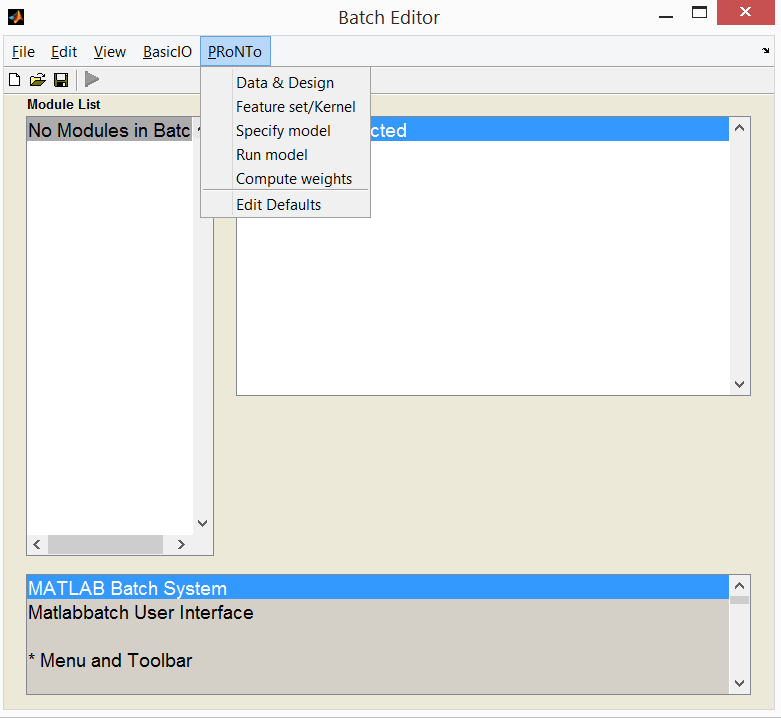
\includegraphics[scale=0.6]{images/Tutorial/mkl/batchmkl.png}
	\caption{Menu PRoNTo in the main {\tt matlabbatch} window.}
	\label{fig:batchmkl}
\end{figure}

%--------------------------------------------------------------

\subsection{Data \& Design}

\begin{itemize}

	\item Click on `Data \& Design' in the PRoNTo menu (Figure \ref{fig:batchDatamkl});
	
	\begin{figure}[!h]
	
	\centering
		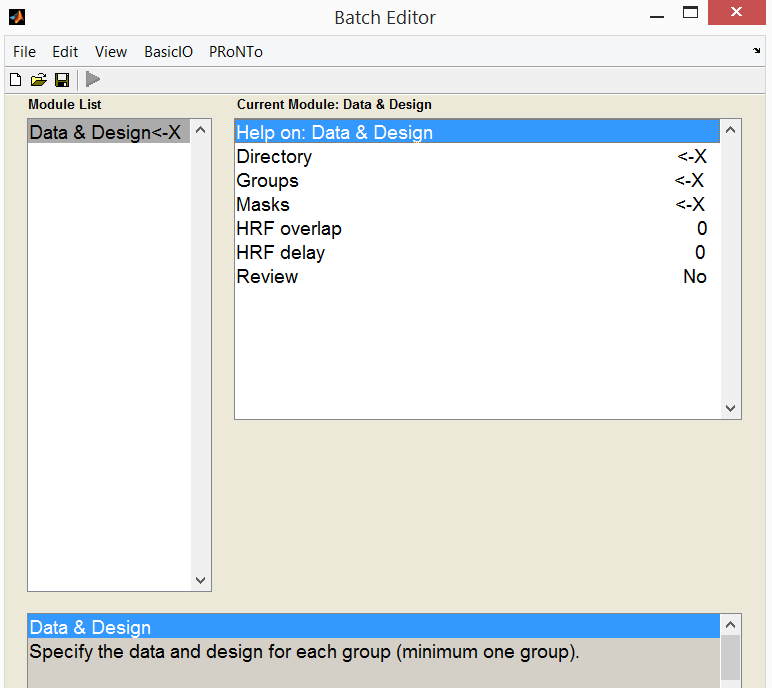
\includegraphics[scale=0.6]{images/Tutorial/mkl/batchDatamkl.png}
	\caption{Data and design module in {\tt matlabbatch}. }
	\label{fig:batchDatamkl}
	
	\end{figure}

	\item In the `Directory' field, select a directory where the `PRT.mat' file will be saved. There are three options to edit all fields in {\tt matlabbatch}: (i) by using the right mouse button and clicking on the current option, (ii) clicking on current button in the window or (iii) by double clicking;
	
	\item In the `Groups' field:
 	
		\begin{itemize}
		
		\item Add one group;
		
		\item In the field `Name', provide a name without spaces to that group, e.g. `G1'; 
		
		\item In the field `Select by', select the `Subjects' option and add one subject;
		
		\item Add on modality for this subject and provide a name, e.g. `fMRI'; define the `Interscan interval' of 2.5 seconds; and in the field `Scans', select all the image files available in the fMRI directory of the Haxby dataset;	
		
		\item In the `Data \& Design' field, choose `Load SPM.mat' option. This file is available with the Haxby dataset on PRoNTo's website\footnote{http://www.mlnl.cs.ucl.ac.uk/pronto/prtdata.html} inside the folder Haxby\_dataset/design/. The batch editor should look similar to the Figure \ref{fig:batchGroupsmkl};	
		
		\begin{figure}[!h]
	\centering
		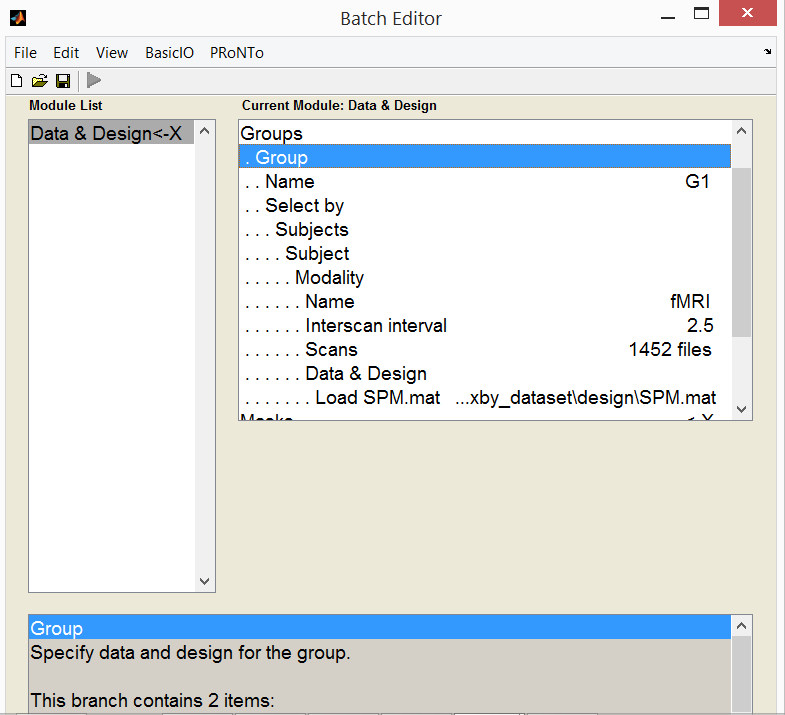
\includegraphics[scale=0.6]{images/Tutorial/mkl/batchGroupsmkl.png}
	\caption{Data and design module in {\tt matlabbatch}. }
	\label{fig:batchGroupsmkl}
	\end{figure}
				
		
		\begin{itemize}
	
			\item In case there is no `SPM.mat' file already available to use, create a new 	design by selecting the option `Specify design'. Choose how many conditions you have, which in this case are 8 conditions (corresponding to the 8 categories of images). The unit in which the onsets/durations are read is `Scans'. Write the names, onsets and durations of each condition (Figure \ref{fig:batchSpecifyDesignmkl});
	
\begin{figure}[!h]
	\centering
		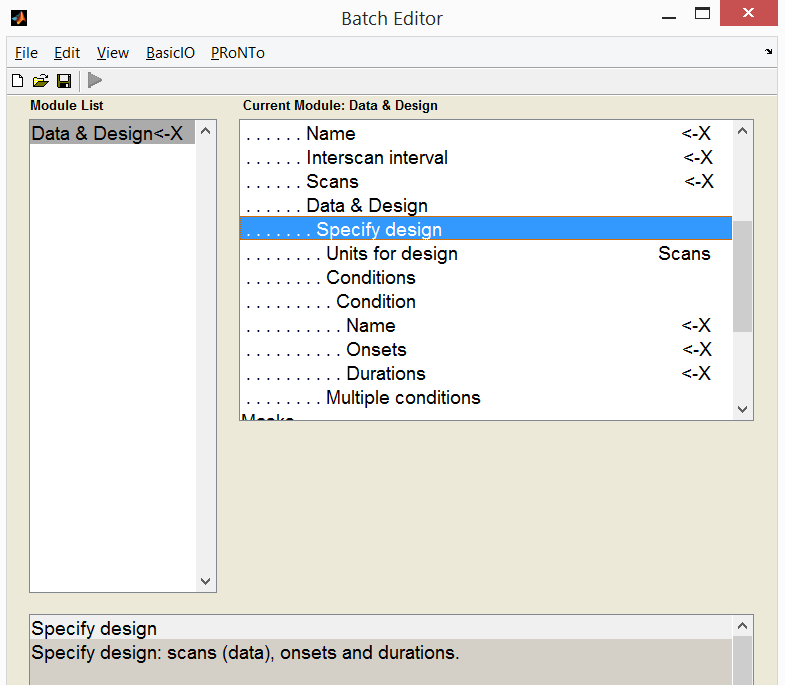
\includegraphics[scale=0.6]{images/Tutorial/mkl/batchSpecifyDesignmkl.png}
	\caption{Data and design module. The `Specify design' option.}
	\label{fig:batchSpecifyDesignmkl}
\end{figure}
	
	\end{itemize}

		\end{itemize}
	
	\item In the `Masks' field, add a new modality and provide the same modality name, `fMRI'; and select the `whole\_brain' mask available in the masks directory of the Haxby dataset. The name of the modality here has to be exactly the same as in `Modalities', otherwise it will not work;
	
	\item Leave the `HRF overlap' and the `HRF delay' options as default;
	
	\item In the `Review' field, select `Yes' if you would like to review your data and design in a separate window. Otherwise, leave as it is, i.e. `No'.


\end{itemize}

%------------------------------------------------------------

\subsection{Feature set / Kernel}

\begin{itemize}
	\item Click on the 'Feature set / Kernel' option on PRoNTo's {\tt matlabbatch} menu (Figure \ref{fig:batchFeaturemkl});
	
	\begin{figure}[!h]
	\centering
		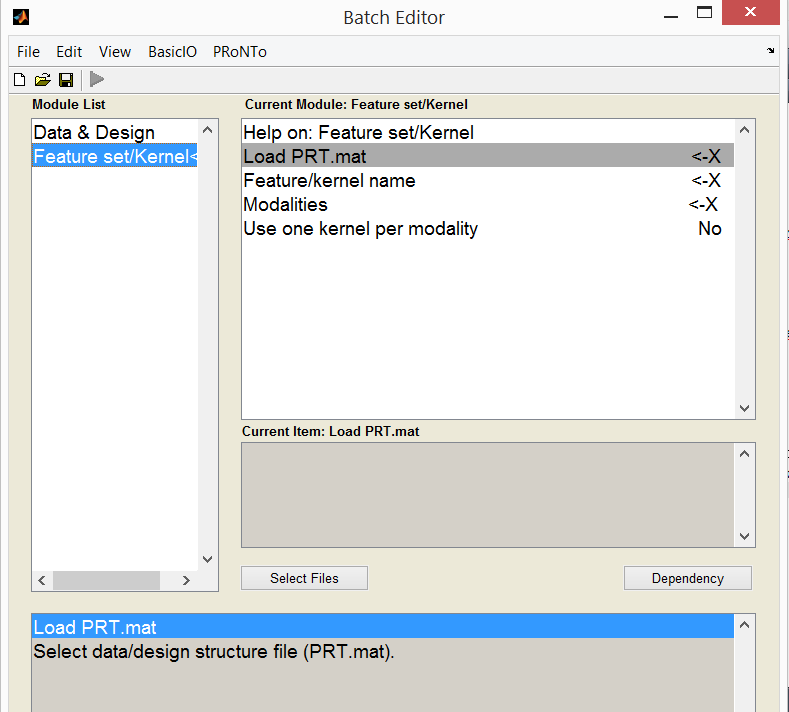
\includegraphics[scale=0.6]{images/Tutorial/mkl/batchFeaturemkl.png}
	\caption{Feature set/Kernel module in {\tt matlabbatch}. }
	\label{fig:batchFeaturemkl}
\end{figure}
	
	\item With `Load PRT.mat' field selected, click on the 'Dependency' button to associate the `PRT.mat' file created in the previous `Data \& Design' step (Figure \ref{fig:batchDependencymkl}) or click on the `Select files' button to browse where `PRT.mat' file was saved;
	
	 	
\begin{figure}[!h]
	\centering
		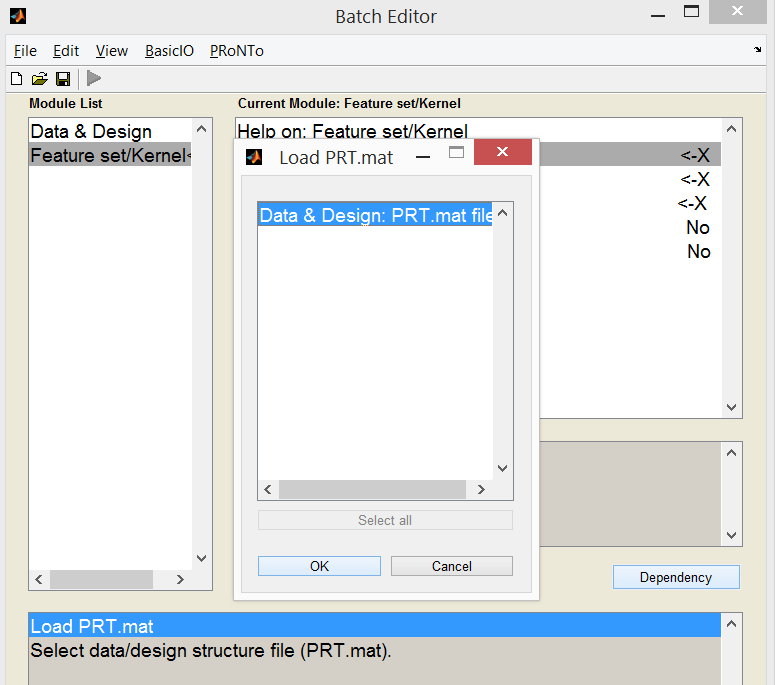
\includegraphics[scale=0.6]{images/Tutorial/mkl/batchDependencymkl.png}
	\caption{Feature set / Kernel module in {\tt matlabbatch}. This window is called to establish a dependency connection with the previous `Data and design' module.}
	\label{fig:batchDependencymkl}
\end{figure}
	
	\item Provide a name to the `Feature/kernel' set, e.g. `HaxbyFeatures';
	
	\item Add one modality and select the modality name with the `Dependency' button\footnote{Or type it in manually, `fMRI', but the name needs to be {\it exactly} the same as the one specified in the `Data \& Design' module.}(Data \& Design:Mod\#1 name);
	
		\begin{itemize}
	
	\item In the `Scans/Conditions' field , select `All scans' option;
	
	\item In the `Voxels to include' field, select `All voxels' option, this means we are not entering an additional second-level mask;
	
			%\begin{itemize}
			%\item This is an optional step. In the `Voxels to include' options, the user can specify a `second-level' mask, which would define regions of interest (ROIs) on which the classification can be performed. In this case, select the `fusiform\_gyrus' mask;
			%\end{itemize}
	
	\item In the `Detrend' field, select `Polynomial detrend' option with order 1;
	
	\item In the `Scale input scans' field, select `No scaling' option;
	
	\item In the `Use atlas to build ROI specific kernels', select an atlas file AAL (named `aal\_79x91x69) available in the PRoNTo directory (PRoNTo/atlas/).
 	
	\end{itemize}
	
\item In the field `Use one kernel per modality', select the `No' option.	

After all this steps, the batch editor should look similar to the one in Figure \ref{fig:batchModalitymkl}.
	
	\begin{figure}[!h]
	\centering
		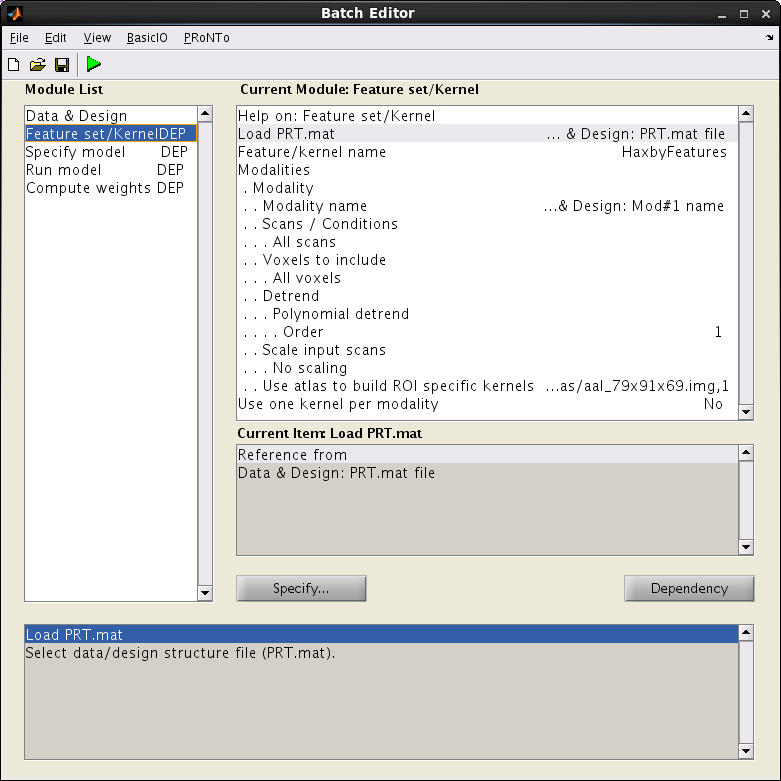
\includegraphics[width=0.75\textwidth]{images/Tutorial/mkl/batchModalitymkl.png}
	\caption{Feature set / Kernel module. Selected parameters in the Modality option.}
	\label{fig:batchModalitymkl}
\end{figure}
	

\end{itemize}

%--------------------------------------------------------

\subsection{Specify model}

\begin{itemize}

\item Click on the `Specify model' option on PRoNTo's {\tt matlabbatch} menu (Figure \ref{fig:batchSpecifyModelmkl});
	
	\begin{figure}[!h]
	\centering
		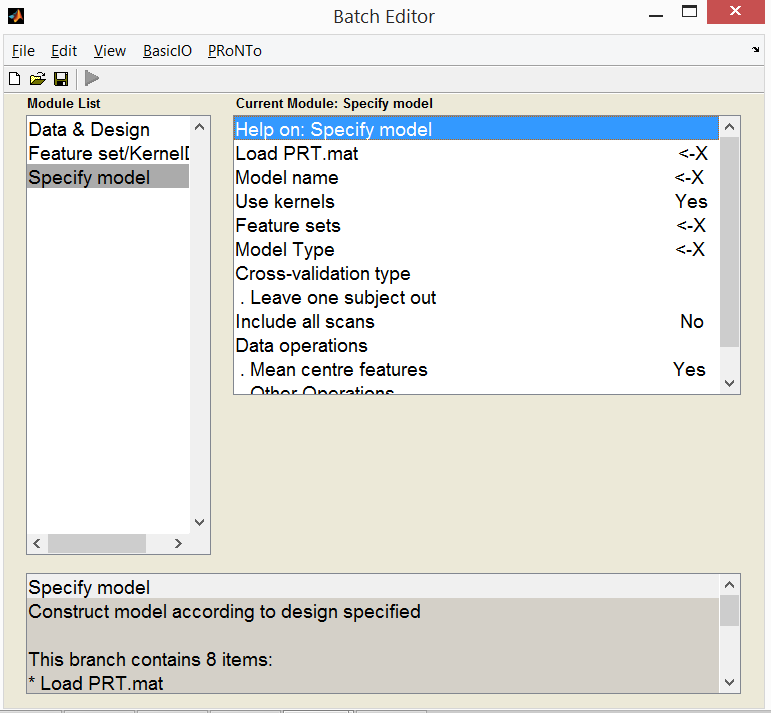
\includegraphics[scale=0.6]{images/Tutorial/mkl/batchSpecifyModelmkl.png}
	\caption{Specify model module in {\tt matlabbatch}.}
	\label{fig:batchSpecifyModelmkl}
\end{figure}
	
	\item With `Load PRT.mat' field selected, click on the `Dependency' button to associate the `PRT.mat' file created in the previous `Feature set / Kernel' step or click on the `Select files' button to browse where `PRT.mat' file was saved;
	
	\item Provide a name to the model, e.g. `mklFacesHouses'; 
	
	\item Leave the `Use kernels' field as it is, i.e. `Yes';
	
	\item In the `Feature sets' field, select the feature set name with the `Dependency' button\footnote{or write it {\it exactly} as previously defined in the `Feature set / Kernel' module (option `Feature set/Kernel: Feature/kernel name'), here `HaxbyFeatures'.};
	
	\item Select the `Classification' model type:
	
		\begin{itemize}
		
		\item Create 2 new classes;
		
		\item For Class (1) write `Faces' on the name field and add one group. Select the group name from the `Data \& Design' module (`Data \& Design:Group\#1 name') with the `Dependency' button\footnote{Or write it {\it exactly} as previously defined in the Data \& Design' module, here `G1'}. Similarly, for Class (2) write `Houses' on the name field and add the group created in the `Data \& Design' module, `G1';	
		
		\item In the `Subjects' field, type `1' (only subject one is selected);
		
		\item In the `Conditions / Scans' field, select the `Specify Conditions' option and add a new condition. Provide a name for this condition, i.e. for Class (1) `Faces' and for Class (2) `Houses'. Note that this name need to be exactly as specified in the `Data \& Design' module: if you simply loaded an `SPM.mat' file for the design, you {\it must} know the names of the conditions;
		
		\item After all this steps, the batch editor should look similar to the Figure \ref{fig:batchClassMKL}	
	
	\begin{figure}[!h]
	\centering
		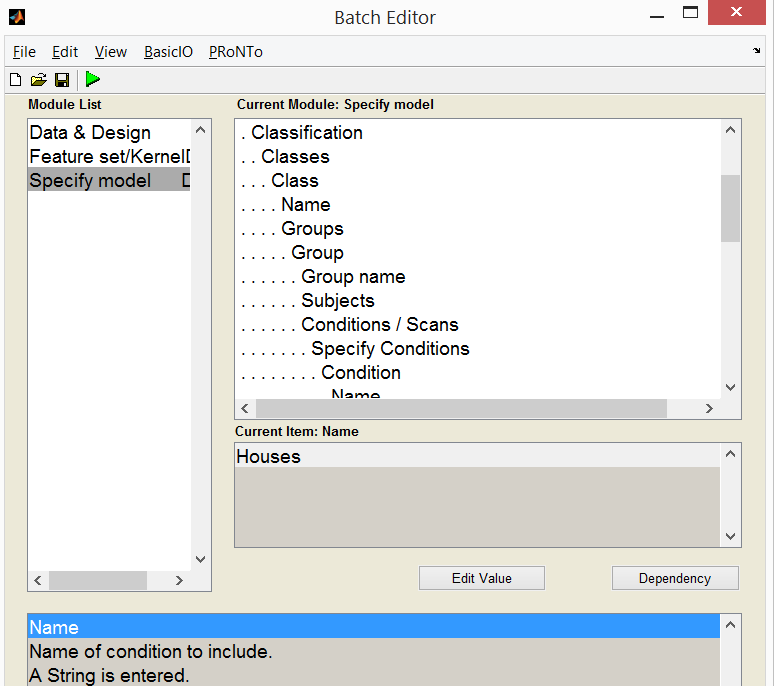
\includegraphics[scale=0.6]{images/Tutorial/mkl/batchClassMKL.png}
	\caption{Specify model module. Selected parameters in the Class option.}
	\label{fig:batchClassMKL}
\end{figure}

		\end{itemize}			
		
	\item In the `Machine' field:
	
	\begin{itemize}
	\item Select `L1 Multi-Kernel Learning' option;	
	
	\item In the `Optimize hyper-parameter' field, select the `Yes' option;
	
	\item In the `Arguments' field, input the hyper-parameters that you wish to use for the hyper-parameter optimization (e.g. [0.01, 0.1, 1, 10, 100, 1000]);
	
	\item In the `Cross validation type for hyper-parameter optimization' (internal loop) field, select the `k-folds CV on blocks' option and on the field `k' input the value 4;
	
	\end{itemize}
	
	\item In the `Cross validation type' (external loop) field, select `Leave one block out' option;
	
	\item Leave the `Include all scans' field as it is, i.e. `No';

	\item In the `Data operations' field:
	
		\begin{itemize}
		\item  Leave the `Mean centre features' field as it is, i.e. `Yes'; 
				
		\item  Click on the `Other Operations' field and select the option `Select Operations', then add a new operation and select the `Normalize samples' option;
		\end{itemize}
	
\end{itemize}

%----------------------------------------------------------

\subsection{Run model}

\begin{itemize}

	\item Click on the 'Run model' option on PRoNTo's {\tt matlabbatch} menu (Figure \ref{fig:batchRunMKL});
	
	\begin{figure}[!h]
	\centering
		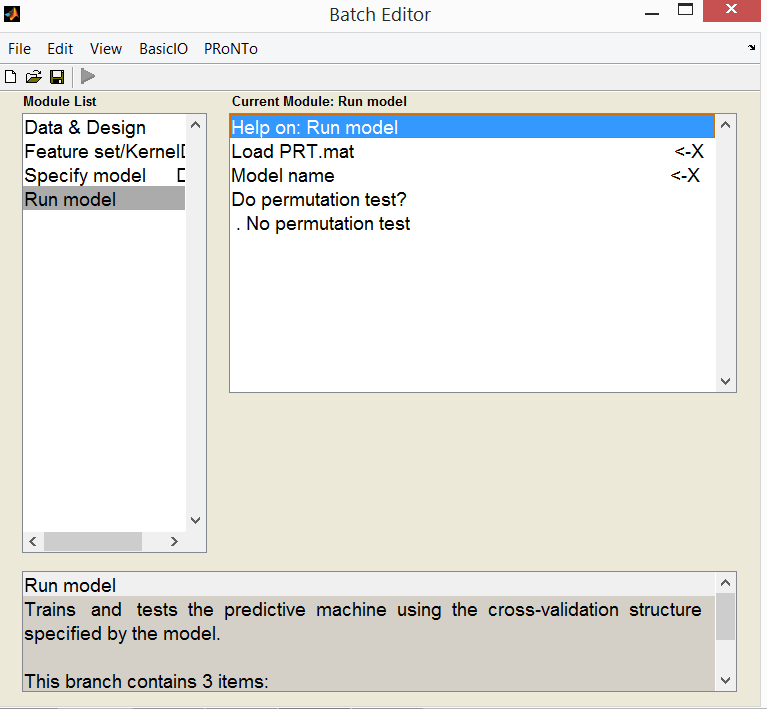
\includegraphics[scale=0.6]{images/Tutorial/mkl/batchRunMKL.png}
	\caption{Run model module in {\tt matlabbatch}.}
	\label{fig:batchRunMKL}
\end{figure}
	
	
	\item  With `Load PRT.mat' field selected, click on the `Dependency' button to associate the `PRT.mat' file created in the previous `Specify model' step;
	
	\item Select the model name from the `Specify model' module with the `Dependency' button\footnote{Or write it {\it exactly} as previously defined in the `Specify model' module, here `mklFacesHouses'};

	\item  Leave the `Do permutation test?' field as it is, i.e. `No permutation test'.

\end{itemize}
%-----------------------------------------------------

\subsection{Compute weights (optional step)}

\begin{itemize}

	\item Click on the `Compute weights' option on PRoNTo's {\tt matlabbatch} menu (Figure \ref{fig:batchWeightsMKL});
	
	\begin{figure}[!h]
	\centering
		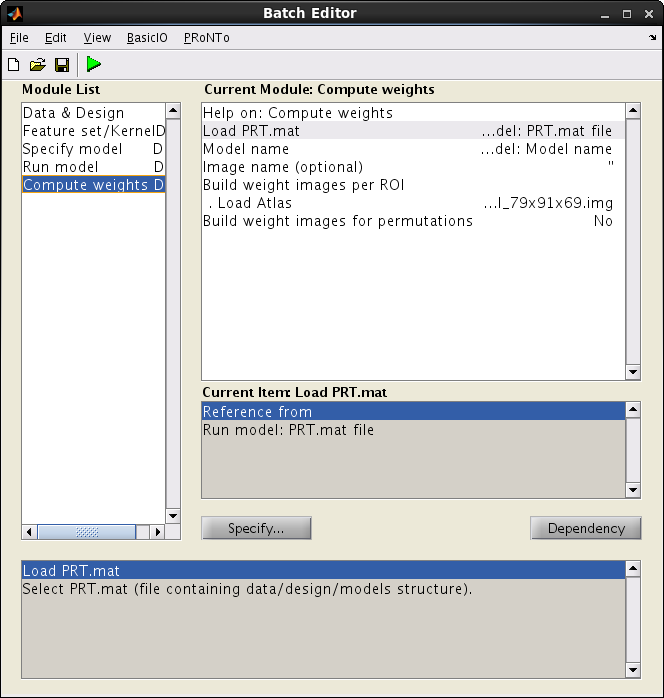
\includegraphics[width=0.75\textwidth]{images/Tutorial/mkl/batchWeightsMKL.png}
	\caption{Compute weights module in {\tt matlabbatch}.}
	\label{fig:batchWeightsMKL}
\end{figure}

	\item With `Load PRT.mat' field selected, click on the `Dependency' button to associate the `PRT.mat' file created in the previous `Run model' step;
	
	\item Select the model name from the `Specify model' module with the `Dependency' button;

	\item It's optional to define a name for the image; 

	\item In the `Build weight images per ROI', load the atlas that was used for building the feature set, which can be found in PRoNTo/atlas/;
	
	\item Leave the `Build weights images for permutations' field as it is, i.e. `No'; 
	

\end{itemize}

Finally, save the batch (e.g. as batch\_run\_all.m) and click on the `Run Batch' option, in the `File menu'. The batch file created can then be opened and edited for further analyses. The results will be the same as those obtained using the GUI (see Section \ref{display_results_MKL}  of this tutorial).
